% Conclusion
\subsection{Training Paradigm}

Centralised Training, Decentralised Execution (CTDE) is a widely used paradigm in Multi-Agent Reinforcement Learning (MARL), addressing coordination challenges among multiple autonomous agents. In this framework, agents are trained with access to \textbf{global state information}, allowing a centralised critic to evaluate joint actions and their overall impact. This shared view enables more stable learning, more accurate credit assignment, and improved coordination during training.

During execution, however, each agent operates independently using only its \textbf{local observations}—without global awareness or centralised control. This design ensures \textbf{scalability}, since adding more agents does not increase reliance on central infrastructure and helps avoid bottlenecks or single points of failure.

\begin{figure}[H]
    \centering
    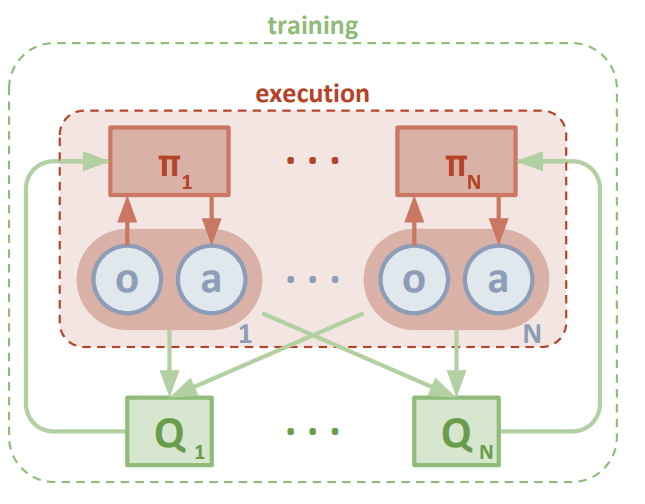
\includegraphics[width=0.7\linewidth]{Figures/CTDE.png}
    \caption{Centralised Training and Decentralised Execution (CTDE) framework.\footcite{lowe2017multiagent}}
    \label{fig:ctde-diagram}
\end{figure}
\footnotetext{Adapted from \cite{lowe2017multiagent}.}

CTDE excels in \textbf{partially observable environments}, where agents cannot fully perceive the environment on their own. Global training data helps agents learn to \textbf{infer hidden information} and develop \textbf{cooperative strategies}, even when each agent sees only a local slice of the world at execution time.

\vspace{0.5em}
\noindent\textbf{MAGAC in the CTDE Framework}

MAGAC aligns naturally with the CTDE paradigm and is highly suitable for the Parking Mesh system. During training, MAGAC employs a \textbf{centralised graph-based critic}, which aggregates observations and actions from all vehicles in the mesh. This enables the critic to model inter-agent dependencies—such as how one vehicle’s detection or relay of a vacancy affects others downstream.

At execution time, MAGAC uses \textbf{decentralised policies}: each vehicle computes its own actions based on \textbf{local sensor data and short-range Bluetooth messages} from neighbouring vehicles. This decentralised execution ensures the Parking Mesh is both scalable and robust—well-suited for dynamic urban environments.

By leveraging global information during training, MAGAC learns strategies that overcome the inherent \textbf{information asymmetry} in real-world parking. It enables vehicles to anticipate and propagate parking availability efficiently, even with limited visibility.

In summary, CTDE offers the ideal balance of central coordination during learning and distributed autonomy during real-world operation. MAGAC’s integration of centralised GNN-based training with decentralised, scalable execution makes it a natural fit for realising the vision of Parking Mesh: a city-wide, cooperative vehicle network that is low-cost, adaptive, and highly effective.
